\chapter{Bacteriën en antibioticaresistentie}\label{ch:g11:antibiotic-resistance}

In 1941 kreeg een politieagent die aan bloedvergiftiging door een schram
lag te sterven, de eerste doses penicilline die ooit bij een patiënt zijn
gebruikt. Hij herstelde binnen enkele dagen --- en kreeg een terugval en
stierf toen de voorraad, moeizaam uit schimmel gewonnen, op was. Binnen
tien jaar werd penicilline per ton gemaakt en werden infecties die
duizenden jaren hadden gedood in een week te genezen. Binnen twintig jaar
kwamen bacteriën waar penicilline niets meer tegen deed in elk ziekenhuis
voor. Dit hoofdstuk gaat over het waarom: hoe bacteriën variëren, hoe een
\omterm{def:g11:antibiotic-resistance:antibiotic}{antibioticum} hen sorteert, en hoe de rekenkunde van een populatie van
miljarden een zeldzame \omterm{def:g11:mutations:mutation}{mutatie} in een probleem voor een hele afdeling
verandert.

\begin{omfigure}
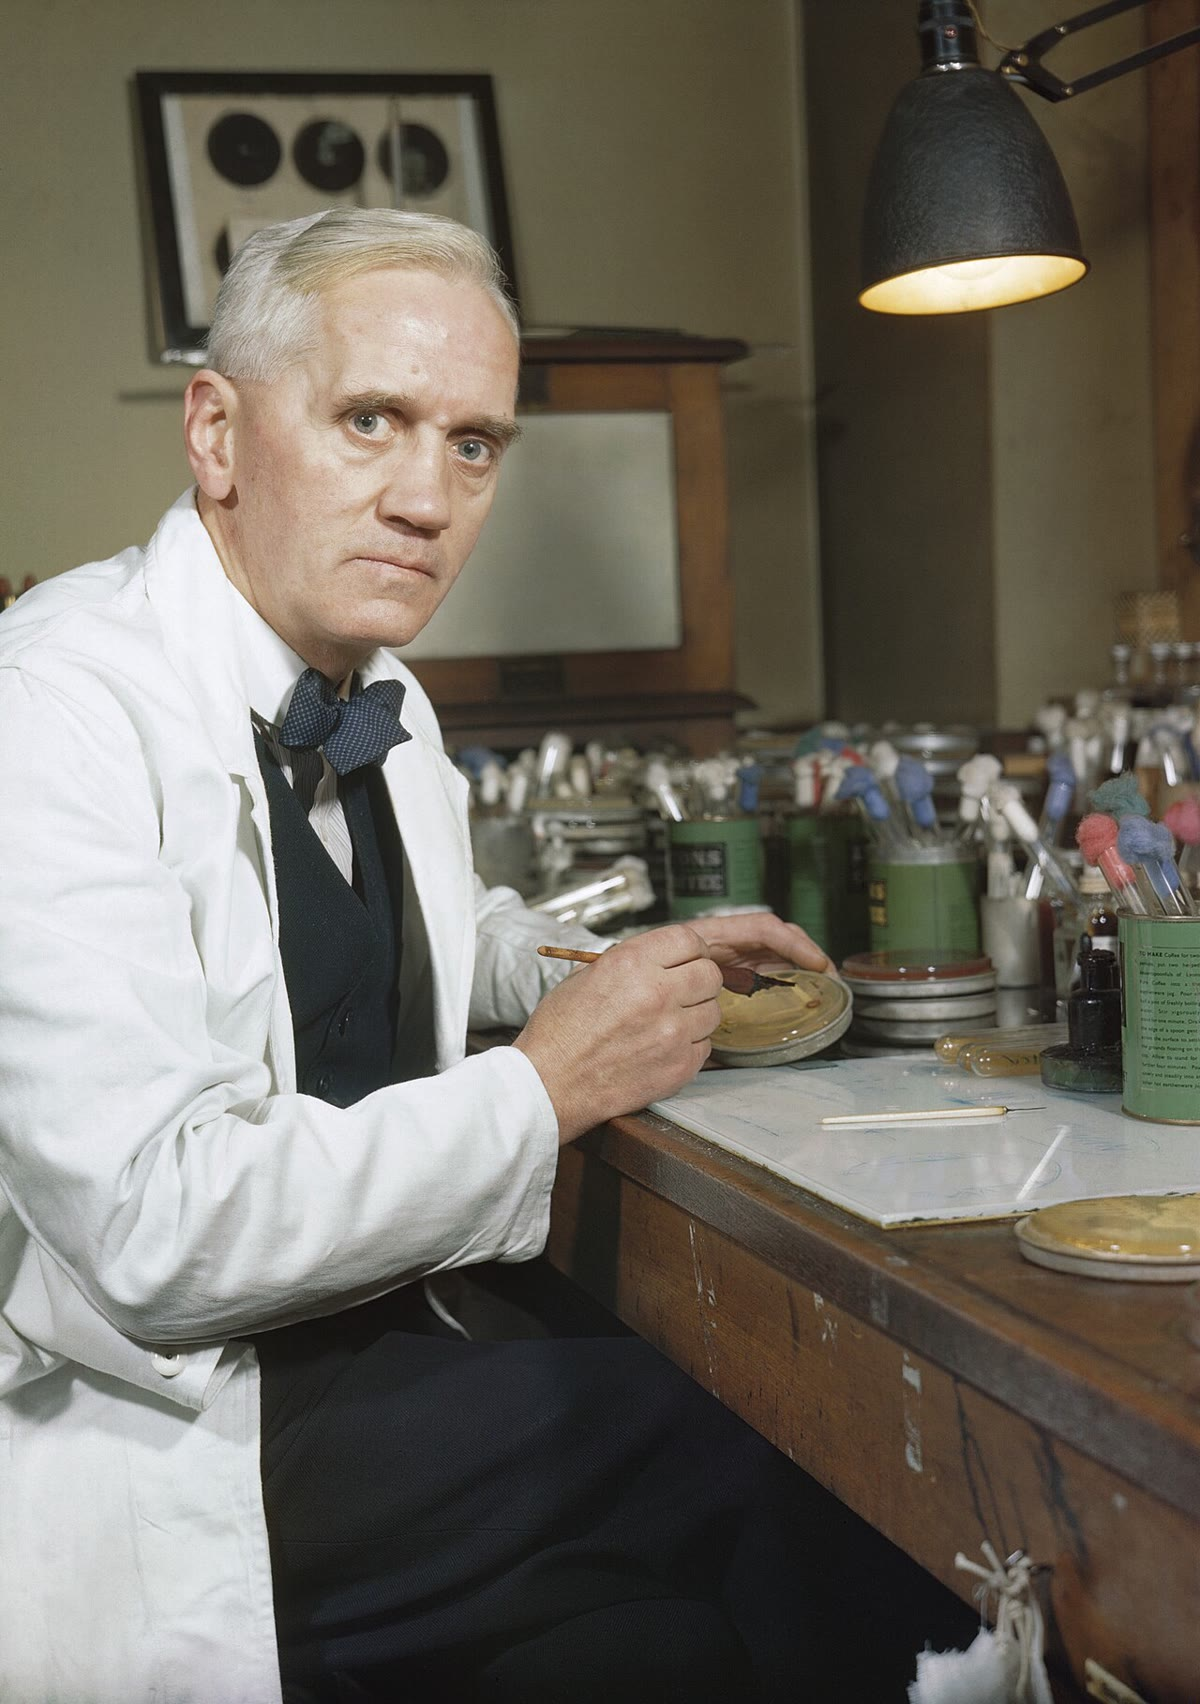
\includegraphics[width=0.4\linewidth]{images/book2/fleming.jpg}

{\small Alexander Fleming aan zijn werktafel in 1943, met de kweekplaten waarop hij vijftien jaar eerder had opgemerkt dat een schimmel de bacteriën eromheen wegnam. Foto, Imperial War Museums, publiek domein.}
\end{omfigure}

\section{Hoe bacteriën variëren}

\begin{proposition}[Voortplanting en variatie bij bacteriën]\label{prop:g11:antibiotic-resistance:variation}
Een bacterie plant zich voort door zich na het kopiëren van haar enige
\omterm{def:g11:cell-cycle-mitosis:chromosome}{chromosoom} in tweeën te delen: de dochters zijn, op kopieerfouten na,
genetisch gelijk aan de moeder --- een \emph{kloon}. In een rijk medium
maakt een deling om de 20 minuten van één \omterm{def:g10:cells-common-unit:cell}{cel} in tien uur een miljard.
Genetische variatie in de kloon komt uit twee bronnen:
\begin{itemize}
  \item \emph{\omterm{def:g11:mutations:mutation}{mutaties}} (\cref{ch:g11:mutations}), zeldzaam per deling
        maar veelvuldig in een populatie van miljarden;
  \item \emph{horizontale genoverdracht}\index{horizontale genoverdracht}:
        \omterm{def:g10:universal-dna:information}{DNA} dat van een andere bacterie wordt ontvangen, van dezelfde of
        van een andere \omterm{def:g10:biodiversity-scales:species}{soort}, meestal als \emph{plasmide} --- een klein
        ringetje \omterm{def:g10:universal-dna:information}{DNA}, los van het \omterm{def:g11:cell-cycle-mitosis:chromosome}{chromosoom}, dat enkele \omterm{def:g10:universal-dna:gene}{genen} draagt en
        via een membraanbrug van \omterm{def:g10:cells-common-unit:cell}{cel} naar \omterm{def:g10:cells-common-unit:cell}{cel} kan overgaan.
\end{itemize}
\end{proposition}
\admitted

\begin{omfigure}
\begin{tikzpicture}[font=\small, >=Stealth]
  % donor
  \draw[thick, fill=omDef!10, rounded corners=12pt] (0,0) rectangle (3,1.5);
  \draw[thick, omDef] (0.4,0.75) .. controls (0.6,1.3) and (2.4,1.3) .. (2.6,0.75) .. controls (2.4,0.2) and (0.6,0.2) .. (0.4,0.75);
  \draw[thick, omThm, fill=omThm!20] (2.2,1.15) circle (0.22);
  \node[anchor=north] at (1.5,-0.1) {donor: heeft de plasmide};
  % recipient
  \draw[thick, fill=omDef!10, rounded corners=12pt] (5,0) rectangle (8,1.5);
  \draw[thick, omDef] (5.4,0.75) .. controls (5.6,1.3) and (7.4,1.3) .. (7.6,0.75) .. controls (7.4,0.2) and (5.6,0.2) .. (5.4,0.75);
  \node[anchor=north] at (6.5,-0.1) {ontvanger};
  % bridge
  \draw[thick, fill=omProp!30] (3,0.55) rectangle (5,0.95);
  \draw[->, thick, omThm] (3.1,0.75) -- (4.9,0.75);
  \node[anchor=north, font=\scriptsize] at (4,-0.6) {een kopie van de plasmide gaat over de brug};
  % result
  \draw[->, thick] (8.4,0.75) -- (9.2,0.75);
  \draw[thick, fill=omDef!10, rounded corners=12pt] (9.5,0) rectangle (12.5,1.5);
  \draw[thick, omDef] (9.9,0.75) .. controls (10.1,1.3) and (11.9,1.3) .. (12.1,0.75) .. controls (11.9,0.2) and (10.1,0.2) .. (9.9,0.75);
  \draw[thick, omThm, fill=omThm!20] (11.7,1.15) circle (0.22);
  \node[anchor=north, align=center] at (11,-0.1) {de ontvanger draagt nu\\ de genen van de plasmide};
  \node[anchor=west, font=\scriptsize, omDef] at (0.2,1.75) {chromosoom};
  \node[anchor=west, font=\scriptsize, omThm] at (2.5,1.75) {plasmide};
\end{tikzpicture}

{\small Horizontale overdracht. Een plasmide --- een klein ringetje \omterm{def:g10:universal-dna:information}{DNA}
dat een weerstandsgen kan dragen --- wordt over een brug van de ene
bacterie naar de andere gekopieerd, die niet van dezelfde \omterm{def:g10:biodiversity-scales:species}{soort} hoeft te
zijn. De ontvanger, en al haar nakomelingen, krijgen het \omterm{def:g10:universal-dna:gene}{gen} in één stap.}
\end{omfigure}

\begin{example}[De rekenkunde van een populatie]\label{ex:g11:antibiotic-resistance:arithmetic}
Een weerstandsmutatie ontstaat ongeveer één keer per $10^8$ delingen. In
een kolf met $10^9$ bacteriën zijn dus, in de delingen die haar hebben
voortgebracht, zo'n tien van zulke \omterm{def:g11:mutations:mutation}{mutaties} opgetreden; in een besmette
wond of een darm, met $10^{12}$ bacteriën, zo'n tienduizend. Elke grote
populatie bacteriën bevat, nog vóór er enig \omterm{def:g11:antibiotic-resistance:antibiotic}{antibioticum} wordt gebruikt,
\omterm{def:g10:cells-common-unit:cell}{cellen} die ertegen bestand zijn --- de stempelplaten van
\cref{ch:g11:mutations} bewezen het.
\end{example}

\section{Antibiotica}

\begin{definition}[Antibioticum]\label{def:g11:antibiotic-resistance:antibiotic}
Een \emph{antibioticum}\index{antibioticum} is een molecuul dat bacteriën
doodt of hun groei stillegt, bij concentraties die voor de \omterm{def:g10:cells-common-unit:cell}{cellen} van de
patiënt onschadelijk zijn, doordat het inwerkt op een structuur of een
proces dat bacteriën wel en menselijke \omterm{def:g10:cells-common-unit:cell}{cellen} niet hebben: penicilline en
haar verwanten blokkeren de bouw van de bacteriewand; streptomycine en
tetracycline blokkeren het bacteriële \omterm{def:g10:cells-common-unit:organelle}{ribosoom}, dat van het onze
verschilt; andere blokkeren de bacteriële \omterm{def:g11:enzymes-and-phenotype:enzyme}{enzymen} van de \omterm{def:g11:dna-replication:replication}{DNA-replicatie}.
De meeste zijn voor het eerst gevonden in schimmels en bodembacteriën,
die ze tegen hun concurrenten maken. Antibiotica hebben geen enkel effect
op virussen, die geen van die aangrijpingspunten hebben.
\end{definition}

\begin{proposition}[Mechanismen van weerstand]\label{prop:g11:antibiotic-resistance:mechanisms}
Een bacterie is \emph{bestand}\index{antibioticaresistentie} tegen een
\omterm{def:g11:antibiotic-resistance:antibiotic}{antibioticum} wanneer zij groeit bij concentraties die haar gevoelige
verwanten stilleggen. Die weerstand heeft een genetische grondslag van
een van enkele typen: een \omterm{def:g10:universal-dna:gene}{gen} voor een \omterm{def:g11:enzymes-and-phenotype:enzyme}{enzym} dat het \omterm{def:g11:antibiotic-resistance:antibiotic}{antibioticum}
afbreekt (penicillinases knippen penicilline doormidden); een \omterm{def:g11:mutations:mutation}{mutatie} die
het aangrijpingspunt van het \omterm{def:g11:antibiotic-resistance:antibiotic}{antibioticum} verandert zodat het middel niet
meer bindt (een veranderd ribosoomeiwit); een pomp die het middel
uitwerpt; een wand die het niet binnenlaat. Elk daarvan is een \omterm{def:g10:universal-dna:gene}{allel} of
een \omterm{def:g10:universal-dna:gene}{gen}, en elk wordt geërfd --- verticaal door de kloon en, als het op
een plasmide zit, horizontaal door de buren.
\end{proposition}
\admitted

\begin{method}[Een antibiogram lezen]\label{met:g11:antibiotic-resistance:antibiogram}
Een \emph{antibiogram} toetst de bacteriën van een patiënt tegelijk tegen
verscheidene \omterm{def:g11:antibiotic-resistance:antibiotic}{antibiotica}.
\begin{enumerate}
  \item Strijk de bacteriën gelijkmatig op een plaat uit; leg er papieren
        schijfjes op die elk met één \omterm{def:g11:antibiotic-resistance:antibiotic}{antibioticum} zijn gedrenkt; laat
        overnacht bebroeden.
  \item Het \omterm{def:g11:antibiotic-resistance:antibiotic}{antibioticum} verspreidt zich uit het schijfje en zijn
        concentratie daalt met de afstand; de bacteriën groeien uit tot
        een tapijt, behalve waar de concentratie hen tegenhoudt: een
        heldere \emph{remmingszone} rond elk schijfje.
  \item Meet de doorsnede van elke zone en vergelijk die met de
        drempelwaarde die voor dat \omterm{def:g11:antibiotic-resistance:antibiotic}{antibioticum} is vastgesteld: een
        doorsnede boven de drempel betekent gevoelig, eronder bestand.
  \item De grootste zones onder de gevoelige uitslagen leiden het
        voorschrift; een schijfje zonder enige zone is een \omterm{def:g11:antibiotic-resistance:antibiotic}{antibioticum}
        waar de stam niets van merkt.
\end{enumerate}
\end{method}

\begin{omfigure}
\begin{tikzpicture}[font=\small]
  \draw[thick, fill=omProp!12] (0,0) circle (3.7);
  \foreach \a/\r/\l in {90/1.3/A, 162/0.9/B, 234/0.0/C, 306/1.6/D, 18/0.55/E} {
    \begin{scope}[shift={(\a:2.0)}]
      \ifdim \r pt > 0pt \draw[fill=white] (0,0) circle (\r); \fi
      \draw[fill=gray!30] (0,0) circle (0.28);
      \node[font=\scriptsize] at (0,0) {\l};
    \end{scope}
  }
  \node[anchor=west, align=left] at (3.8,1.6) {A: zone \qty{26}{mm}, drempel 17: gevoelig};
  \node[anchor=west, align=left] at (3.8,0.9) {B: zone \qty{18}{mm}, drempel 20: bestand};
  \node[anchor=west, align=left] at (3.8,0.2) {C: geen zone: bestand};
  \node[anchor=west, align=left] at (3.8,-0.5) {D: zone \qty{32}{mm}, drempel 22: gevoelig};
  \node[anchor=west, align=left] at (3.8,-1.2) {E: zone \qty{11}{mm}, drempel 15: bestand};
  \node[anchor=north, align=center] at (0,-3.9) {tapijt van de bacteriën van de patiënt;\\ witte schijven van heldere voedingsbodem rond de antibioticumschijfjes};
\end{tikzpicture}

{\small Een afgelezen antibiogram. Elk schijfje bevat één \omterm{def:g11:antibiotic-resistance:antibiotic}{antibioticum}; de
heldere zone is waar de bacteriën niet konden groeien. Vergeleken met de
drempel van elk middel delen de doorsnedes de stam in als gevoelig voor A
en D, en bestand tegen B, C en E.}
\end{omfigure}

\begin{omfigure}
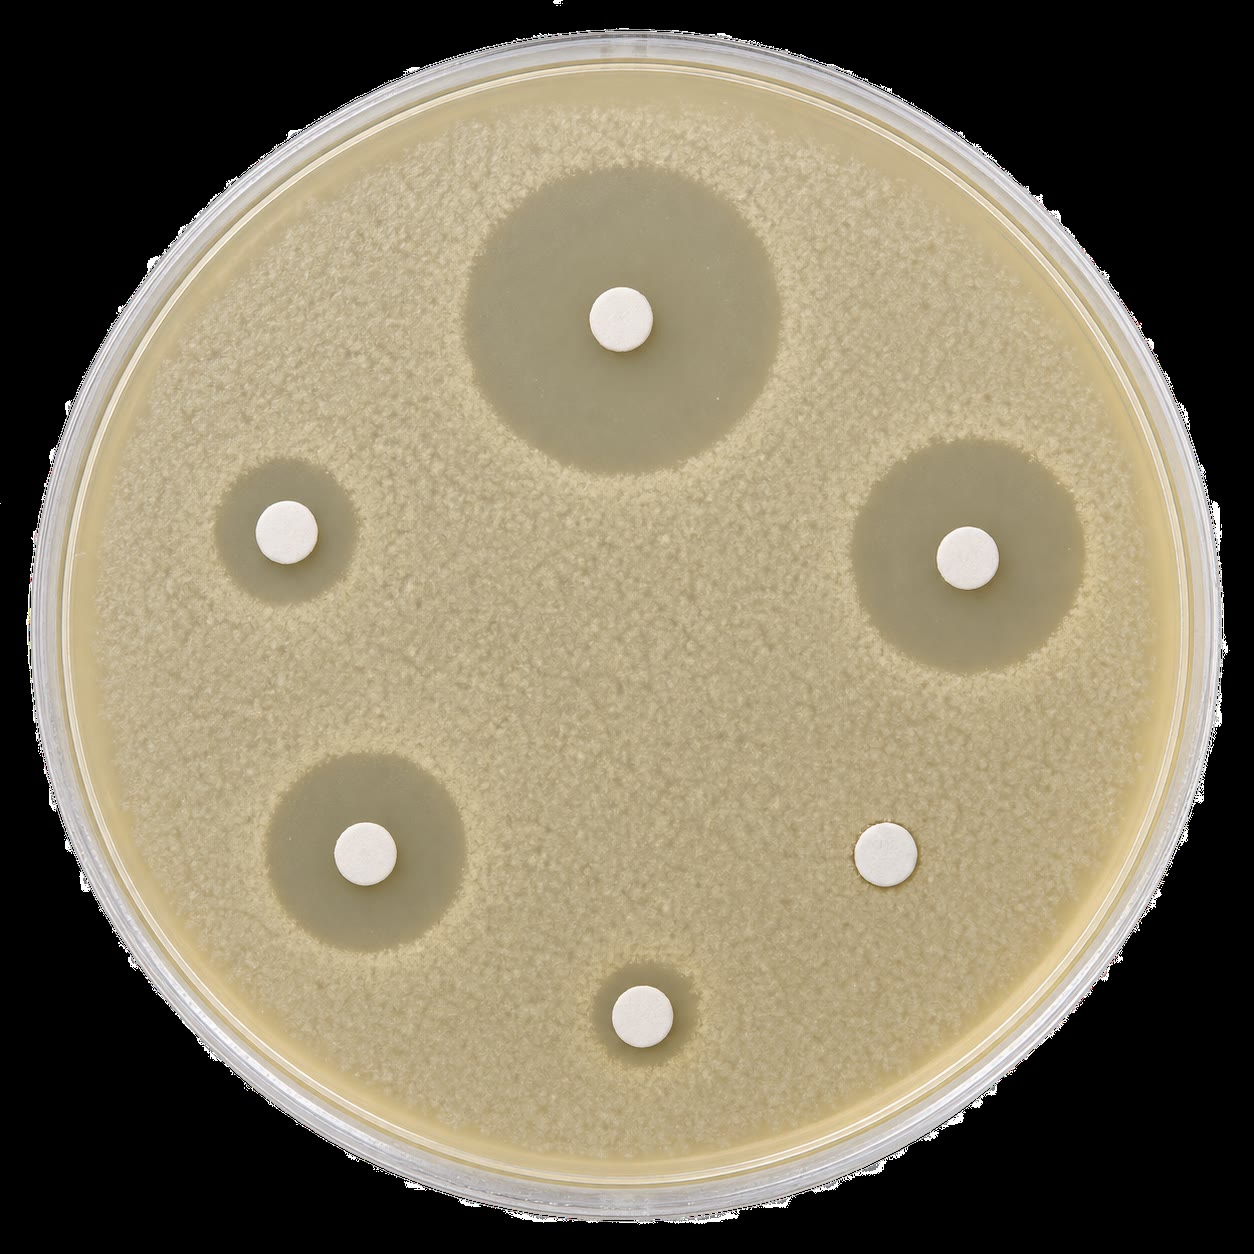
\includegraphics[width=0.44\linewidth]{images/book2/ai/g11-antibiogram-plate.jpg}

{\small Een antibiogramplaat na een nacht bebroeden: een tapijt bacteriën,
en rond elk antibioticumschijfje een heldere zone waarvan de grootte de
gevoeligheid van de stam meet. Eén schijfje heeft geen zone.}
\end{omfigure}

\section{Hoe weerstand zich verbreidt}

\begin{proposition}[Selectie door het antibioticum]\label{prop:g11:antibiotic-resistance:selection}
Een \omterm{def:g11:antibiotic-resistance:antibiotic}{antibioticum} schept geen bestendige bacteriën; het
\emph{selecteert} ze. In een populatie waarin enkele \omterm{def:g10:cells-common-unit:cell}{cellen} een
weerstandsallel dragen, doodt of stopt het middel de gevoelige
meerderheid en laat het de bestendige enkelingen zich zonder concurrentie
vermenigvuldigen: binnen enkele dagen is de populatie bestendig. Hoe meer
een \omterm{def:g11:antibiotic-resistance:antibiotic}{antibioticum} wordt gebruikt --- bij patiënten, bij dieren, in het
milieu --- des te vaker dat sorteren gebeurt, en des te bestendiger de
bacteriën van een ziekenhuis, een boerderij of een land worden. Een kuur
die niet wordt afgemaakt en die de gevoeligste \omterm{def:g10:cells-common-unit:cell}{cellen} doodt en de minst
gevoelige spaart, selecteert nog het doeltreffendst van al.
\end{proposition}
\begin{proof}[Bewijsmateriaal]
De stempelplaten van Lederberg lieten zien dat de bestendige \omterm{def:g10:cells-common-unit:cell}{cellen} er
vóór de blootstelling al waren. Kweken die een week lang in oplopende
concentraties van een \omterm{def:g11:antibiotic-resistance:antibiotic}{antibioticum} groeien, worden op het eind bestand
tegen honderd keer de begindosis, en hun weerstand is erfelijk en aan
bepaalde \omterm{def:g11:mutations:mutation}{mutaties} toe te schrijven. Landen die per inwoner de meeste
\omterm{def:g11:antibiotic-resistance:antibiotic}{antibiotica} gebruiken, hebben de hoogste aandelen bestendige stammen;
ziekenhuisafdelingen die hun gebruik terugbrengen, zien de weerstand over
maanden dalen. Een stam van de huidbacterie \emph{Staphylococcus aureus}
die bestand is tegen penicilline verscheen binnen vier jaar na de
invoering van het middel en vormt nu de meeste ziekenhuisstammen; de stam
die bestand is tegen het vervangende middel volgde die vervanging twee
jaar later.
\end{proof}

\begin{omfigure}
\begin{tikzpicture}
\begin{axis}[
  width=0.88\linewidth, height=5.8cm,
  axis x line=bottom, axis y line=left,
  xmin=0, xmax=6, ymin=0, ymax=110,
  xlabel={dagen behandeling}, ylabel={bacteriën (\% van het begin)},
  xlabel style={font=\small, at={(axis description cs:0.5,-0.12)}, anchor=north},
  ylabel style={font=\small},
  tick label style={font=\small}, xtick={0,1,2,3,4,5,6}, ytick={0,25,50,75,100},
  legend style={at={(0.5,-0.3)}, anchor=north, legend columns=3, font=\small, draw=none},
  clip=false,
]
\addplot[thick, omDef] coordinates {(0,100) (0.5,45) (1,15) (1.5,5) (2,1.5) (3,0.2) (4,0.05) (5,0.01) (6,0)};
\addplot[thick, omThm] coordinates {(0,0.001) (1,0.01) (2,0.1) (3,1) (4,8) (5,40) (6,100)};
\addplot[thick, omMeth, dashed] coordinates {(0,100) (0.5,45) (1,15) (1.5,5) (2,1.5) (3,1.2) (4,9) (5,48) (6,100)};
\legend{gevoelige cellen, bestendige cellen (van één op $10^5$), totaal als de behandeling op dag 3 stopt}
\end{axis}
\end{tikzpicture}

{\small Selectie tijdens een antibioticumkuur. De gevoelige \omterm{def:g10:cells-common-unit:cell}{cellen} (blauw)
worden binnen enkele dagen gedood; de bestendige enkelingen (rood)
vermenigvuldigen zich zonder tegenstand en vormen aan het eind van de week
de hele populatie. Stopt de patiënt op dag 3, dan groeien de overlevenden
weer aan --- nu vrijwel allemaal bestendig.}
\end{omfigure}

\begin{example}[Van één cel tot een hele afdeling]\label{ex:g11:antibiotic-resistance:ward}
Een patiënt die met penicilline wordt behandeld, draagt onder $10^{10}$
bacteriën honderd bestendige. In drie dagen zijn de gevoelige verdwenen
en heeft de bestendige kloon hun plaats ingenomen: $10^{10}$ bestendige
\omterm{def:g10:cells-common-unit:cell}{cellen}. Op de handen van een verpleegkundige, op een bedhek, in de
volgende patiënt gaat de kloon verder --- en zit haar weerstandsgen op
een plasmide, dan geeft zij het onderweg aan andere \omterm{def:g10:biodiversity-scales:species}{soorten} door. Nergens
in die reeks moest het \omterm{def:g11:antibiotic-resistance:antibiotic}{antibioticum} op het \omterm{def:g10:universal-dna:information}{DNA} inwerken; het nam alleen de
concurrentie weg.
\end{example}

\section{Antibiotica werkzaam houden}

\begin{proposition}[Gevolgen en antwoorden]\label{prop:g11:antibiotic-resistance:consequences}
Infecties met bestendige bacteriën duren langer, kosten meer en zijn
vaker dodelijk; sommige stammen weerstaan nu elk beschikbaar middel.
Omdat de weerstand door het gebruik wordt aangedreven, is het antwoord
\omterm{def:g11:antibiotic-resistance:antibiotic}{antibiotica} minder en beter te gebruiken: alleen bij bacteriële infecties
(nooit bij virale verkoudheid en griep), waar mogelijk gekozen na een
antibiogram, in de volle dosis en gedurende de volle kuur, met het meest
gerichte middel dat werkt; hun gebruik in de veehouderij te beperken;
infectie te voorkomen (hygiëne, inenting) zodat er minder kuren nodig
zijn; en dragers van bestendige stammen in ziekenhuizen te isoleren.
Nieuwe \omterm{def:g11:antibiotic-resistance:antibiotic}{antibiotica} kopen tijd; de rekenkunde van de selectie waarborgt
dat er tegen elk ervan weerstand zal verschijnen.
\end{proposition}
\admitted

\begin{remark}[Evolutie in een week]\label{rem:g11:antibiotic-resistance:evolution}
\omterm{def:g11:mutations:mutation}{Mutatie} die willekeurig variatie levert, een omgeving die haar sorteert,
en nakomelingen van de overlevenden die het verschil erven: de bacteriën
van dit hoofdstuk doorlopen in een week het proces dat het laatste jaar
over miljoenen jaren voor walvissen en eiken zal beschrijven.
\omterm{prop:g11:antibiotic-resistance:mechanisms}{Antibioticaresistentie} is evolutie door natuurlijke selectie, in
werkelijke tijd waargenomen, met de mens als selecterende kracht --- en de
duidelijkste demonstratie dat het proces geen theorie over het verleden
is, maar een feit over elke populatie die varieert en zich voortplant.
\end{remark}

\section{Oefeningen}

\begin{exercise}[$\star$]\label{exo:g11:antibiotic-resistance:1}
Noem de twee bronnen van genetische variatie in een populatie bacteriën.
\end{exercise}

\begin{exercise}[$\star$]\label{exo:g11:antibiotic-resistance:2}
Wat is een \omterm{def:g11:antibiotic-resistance:antibiotic}{antibioticum}, en waarom schaadt het bacteriën maar niet de
\omterm{def:g10:cells-common-unit:cell}{cellen} van de patiënt? Waarom helpt het niet tegen een verkoudheid?
\end{exercise}

\begin{exercise}[$\star$]\label{exo:g11:antibiotic-resistance:3}
Geef drie mechanismen waarmee een bacterie een \omterm{def:g11:antibiotic-resistance:antibiotic}{antibioticum} kan
weerstaan.
\end{exercise}

\begin{exercise}[$\star$]\label{exo:g11:antibiotic-resistance:4}
In de antibiogramfiguur geeft een nieuw schijfje F een zone van
\qty{20}{mm} bij een drempel van \qty{18}{mm}. Gevoelig of bestand? Welk
\omterm{def:g11:antibiotic-resistance:antibiotic}{antibioticum} van A tot en met F zou je voorschrijven?
\end{exercise}

\begin{exercise}[$\star$]\label{exo:g11:antibiotic-resistance:5}
Veroorzaakt een \omterm{def:g11:antibiotic-resistance:antibiotic}{antibioticum} weerstandsmutaties? Verantwoord dat met de
proef uit \cref{ch:g11:mutations}.
\end{exercise}

\begin{exercise}[$\star\star$]\label{exo:g11:antibiotic-resistance:6}
Hoeveel bacteriën zijn er na 10 uur, uitgaande van één bacterie die zich
om de 20 minuten deelt? Hoeveel bestendige \omterm{def:g10:cells-common-unit:cell}{cellen} bevat de kweek
waarschijnlijk, als weerstand één keer per $10^8$ delingen ontstaat?
\end{exercise}

\begin{exercise}[$\star\star$]\label{exo:g11:antibiotic-resistance:7}
Op welke dag worden bestendige \omterm{def:g10:cells-common-unit:cell}{cellen} volgens de selectiefiguur de
meerderheid van het totaal? Hoe groot is de totale populatie op dag 6 in
het geval van de streepjeslijn, en waaruit bestaat zij?
\end{exercise}

\begin{exercise}[$\star\star$]\label{exo:g11:antibiotic-resistance:8}
Leg uit waarom een weerstandsgen op een plasmide zich sneller verbreidt
dan een \omterm{def:g10:universal-dna:gene}{gen} op het \omterm{def:g11:cell-cycle-mitosis:chromosome}{chromosoom}.
\end{exercise}

\begin{exercise}[$\star\star$]\label{exo:g11:antibiotic-resistance:9}
Een patiënt voelt zich na drie dagen van een kuur van zeven dagen beter
en stopt. Leg met de figuur uit wat er de volgende dagen gebeurt en
waarom de terugval moeilijker te behandelen is.
\end{exercise}

\begin{exercise}[$\star\star$]\label{exo:g11:antibiotic-resistance:10}
Waarom is het aandeel bestendige stammen in ziekenhuizen hoger dan in de
algemene bevolking?
\end{exercise}

\begin{exercise}[$\star\star$]\label{exo:g11:antibiotic-resistance:11}
Leg uit waarom een \omterm{def:g11:mutations:mutation}{mutatie} die een ribosoomeiwit verandert een bacterie
bestand kan maken tegen streptomycine, en waarom zo'n bacterie vaak wat
langzamer groeit dan haar gevoelige verwanten.
\end{exercise}

\begin{exercise}[$\star\star\star$]\label{exo:g11:antibiotic-resistance:12}
Er worden twee \omterm{def:g11:antibiotic-resistance:antibiotic}{antibiotica} met verschillende aangrijpingspunten samen
gegeven. Schat de kans dat een \omterm{def:g10:cells-common-unit:cell}{cel} door onafhankelijke \omterm{def:g11:mutations:mutation}{mutaties} tegen
beide bestand is (elk één op $10^8$), en leg uit waarom bij trage, lange
infecties zoals tuberculose een combinatiebehandeling wordt gebruikt.
\end{exercise}

\begin{exercise}[$\star\star\star$]\label{exo:g11:antibiotic-resistance:13}
Een boerderij mengt lage doses van een \omterm{def:g11:antibiotic-resistance:antibiotic}{antibioticum} door het veevoer om
de groei te versnellen. Voorspel de gevolgen voor de bacteriën van de
dieren, voor de medewerkers van de boerderij en voor de geneeskunde, met
behulp van selectie en horizontale overdracht.
\end{exercise}

\begin{exercise}[$\star\star\star$]\label{exo:g11:antibiotic-resistance:14}
Een afdeling halveert haar antibioticumvoorschriften; binnen een jaar
daalt het aandeel bestendige stammen. Leg uit waarom weerstand kan
teruglopen, met behulp van de prijs die de weerstand de bacterie kost en
van de concurrentie.
\end{exercise}

\begin{exercise}[$\star\star\star$]\label{exo:g11:antibiotic-resistance:15}
"Bacteriën worden bestendig omdat zij aan het \omterm{def:g11:antibiotic-resistance:antibiotic}{antibioticum} wennen."
Herschrijf die zin correct, in een korte alinea, met \omterm{def:g11:mutations:mutation}{mutatie}, selectie en
erfelijkheid.
\end{exercise}

\section{Probleem: De afdeling}

\begin{problem}[{Weekendprobleem --- een uitbraak op een
ziekenhuisafdeling gevolgd vanaf één gemuteerde cel: de rekenkunde van
een kolonie, een afgelezen antibiogram, een afgebroken kuur, en het beleid
dat de verspreiding stopt}]
\label{pb:g11:antibiotic-resistance:1}
De wond van een patiënt is besmet met $10^{10}$ bacteriën van één \omterm{def:g10:biodiversity-scales:species}{soort}.
De bacteriën delen zich om de 30 minuten; een \omterm{def:g11:mutations:mutation}{mutatie} die weerstand tegen
het \omterm{def:g11:antibiotic-resistance:antibiotic}{antibioticum} amoxicilline geeft, treedt één keer per $10^8$ delingen
op. Het \omterm{def:g11:antibiotic-resistance:antibiotic}{antibioticum} doodt elke 6 uur 90\% van de gevoelige \omterm{def:g10:cells-common-unit:cell}{cellen} en
raakt de bestendige \omterm{def:g10:cells-common-unit:cell}{cellen} niet, die zich blijven delen.

\medskip
\noindent\textbf{Deel I --- Vóór de behandeling.}
\begin{enumerate}
  \item Hoeveel delingen hebben de $10^{10}$ bacteriën uit de eerste \omterm{def:g10:cells-common-unit:cell}{cel}
        voortgebracht? (Tel het aantal \omterm{def:g10:cells-common-unit:cell}{cellen}.)
  \item Schat het aantal bestendige \omterm{def:g10:cells-common-unit:cell}{cellen} dat er vóór enig \omterm{def:g11:antibiotic-resistance:antibiotic}{antibioticum}
        aanwezig is.
  \item Leg uit waarom de infectie van de patiënt op het antibiogram toch
        als "gevoelig" wordt beschreven.
  \item Het antibiogram toont zones van \qty{24}{mm} voor amoxicilline
        (drempel 17), \qty{12}{mm} voor erytromycine (drempel 20) en geen
        zone voor penicilline. Leg de drie uitslagen uit.
  \item De arts schrijft 7 dagen amoxicilline voor. Waarom geen
        penicilline, en waarom niet het middel met de grootste zone als
        een ervan groter was geweest?
\end{enumerate}

\medskip
\noindent\textbf{Deel II --- Tijdens de behandeling.}
\begin{enumerate}[resume]
  \item Hoeveel gevoelige \omterm{def:g10:cells-common-unit:cell}{cellen} blijven er na 1 dag over? En na 3 dagen?
  \item Hoeveel bestendige \omterm{def:g10:cells-common-unit:cell}{cellen} zijn er na 1 dag, uitgaande van je
        antwoord op vraag 2 en als zij zich zonder beperking om de 30
        minuten verdubbelen? (Gebruik $2^{48} \approx \num{2.8e14}$.)
        Waarom is dat getal onrealistisch, en wat begrenst het?
  \item Stel dat de bestendige kloon beperkt is tot de ruimte die de
        gevoelige \omterm{def:g10:cells-common-unit:cell}{cellen} vrijmaken, zodat hij niet boven $10^{10}$ kan
        komen. Wanneer vult hij die ruimte ruwweg?
  \item Schets, of beschrijf, de krommen van de gevoelige, de bestendige
        en alle \omterm{def:g10:cells-common-unit:cell}{cellen} over de 7 dagen.
  \item In werkelijkheid ruimt het afweersysteem van de patiënt de
        laatste paar miljoen \omterm{def:g10:cells-common-unit:cell}{cellen} van welke \omterm{def:g10:biodiversity-scales:species}{soort} dan ook binnen enkele
        dagen op. Leg uit waarom de afloop ervan afhangt of de bestendige
        kloon sneller groeit dan het afweersysteem hem opruimt.
\end{enumerate}

\medskip
\noindent\textbf{Deel III --- De afgebroken kuur.}
\begin{enumerate}[resume]
  \item De patiënt stopt na 2 dagen, omdat hij zich goed voelt. Hoeveel
        gevoelige \omterm{def:g10:cells-common-unit:cell}{cellen} blijven er over, en welk deel van de
        overgebleven populatie is bestendig?
  \item De bacteriën groeien de volgende dagen weer aan tot $10^{10}$.
        Welk deel is nu bestendig, als bestendige en gevoelige \omterm{def:g10:cells-common-unit:cell}{cellen}
        even snel groeien?
  \item De patiënt krijgt een terugval en krijgt opnieuw amoxicilline.
        Voorspel het resultaat.
  \item Een antibiogram van de terugval toont geen zone voor
        amoxicilline. Verklaar de verandering ten opzichte van het eerste
        antibiogram.
  \item Het weerstandsgen zit op een plasmide. Welk extra risico brengt
        dat voor de afdeling mee?
\end{enumerate}

\medskip
\noindent\textbf{Deel IV --- Het beleid van de afdeling.}
De afdeling behandelt 400 patiënten per jaar met amoxicilline; 30\% van
de infecties die op de afdeling worden gevonden is nu bestendig, tegen
5\% in de stad.
\begin{enumerate}[resume]
  \item Verklaar het verschil tussen de afdeling en de stad in termen van
        selectiedruk.
  \item De afdeling besluit: een antibiogram vóór elk voorschrift, volle
        kuren, handhygiëne, en isolatie van dragers van bestendige
        stammen. Zeg op welk mechanisme uit dit hoofdstuk elke maatregel
        inwerkt.
  \item Na twee jaar is de weerstand op de afdeling 12\%. Leg uit waarom
        zij is gedaald, en waarom zij niet tot 5\% is teruggekeerd.
  \item Waarom zou een nieuw \omterm{def:g11:antibiotic-resistance:antibiotic}{antibioticum}, op de afdeling ingevoerd, het
        probleem niet langer dan enkele jaren oplossen?
  \item Geef het resultaat: het aantal bestendige \omterm{def:g10:cells-common-unit:cell}{cellen} dat de wond
        droeg vóór enig middel, de dag waarop zij haar erfden, en de ene
        gewoonte van de patiënt die een geneesbare infectie in een
        uitbraak veranderde.
\end{enumerate}
\end{problem}
